%-------------------------------------------------------------------------------
%	EMPIEZA CAPITULO
%-------------------------------------------------------------------------------

\chapter{Nociones de control adaptable}

    El control adaptable es la combinación de una ley de control lineal con un algoritmo de identificación en linea.

    \begin{figure}
        \centering
        \resizebox{0.8\textwidth}{!}{
        \tikzstyle{block} = [draw, rectangle, minimum height=4.5em, minimum width=4em]

        \begin{tikzpicture}[auto, scale=1, node distance=3.2cm, >=latex']
            \node [input, name=entrada] {};
            \node [sum, right of=entrada] (suma) {$+$};
            \node [block, right of=suma] (cont) {Controlador};
            \node [block, right of=cont] (planta) {Planta};
            \node [output, right of=planta] (salida) {};
            \node [block, align=center, below of=planta] (ident) {Algoritmo \\ de \\ Identificación};
            \node [block, below of=ident] (retro) {$-1$};

            \draw [->] (entrada) -- node[name=x] {$\hat{r}(s)$} (suma);
            \draw [->] (suma) -- node[name=e] {$e$} (cont);
            \draw [->] (cont) -- node[name=u] {$u$} (planta);
            \draw [->] (planta) -- node[name=y] {$\hat{y}(s)$} (salida);
            \draw [->] (y) |- (retro);
            \draw [->] (y) |- (ident);
            \draw [->] (u) |- (ident);
            \draw [->] (ident.south) -| (cont.south);
            \draw [->] (retro) -| (suma);
        \end{tikzpicture}}
        \caption{\label{dia:adap1}Sistema con un esquema de control adaptable.}
    \end{figure}

    Para abordar este tipo de controlador necesitamos estudiar primero los conceptos de regresor lineal, algoritmo de identificacion y prueba de convergencia con estabilidad.

%-------------------------------------------------------------------------------
%	EMPIEZA SECCION
%-------------------------------------------------------------------------------
    \newpage
    \section{Regresor lineal}

        Consideremos un sistema lineal, invariante en el tiempo, representado por la siguiente ecuación diferencial ordinaria:

        \begin{equation} \label{eq:adap1}
            M \left( \frac{d}{dt} \right) y(t) = N \left( \frac{d}{dt} \right) u(t)
        \end{equation}

        la cual es equivalente al diagrama de bloques de la figura~\ref{dia:adap2}.

        \begin{marginfigure}
            \centering
            \resizebox{\textwidth}{!}{
                \tikzstyle{block} = [draw, rectangle, minimum height=3em, minimum width=4em]

                \begin{tikzpicture}[auto, node distance=2cm, >=latex']
                    \node [input, name=entrada] {};
                    \node [block, right of=entrada] (planta) {$\frac{N(s)}{M(s)}$};
                    \node [output, right of=planta] (salida) {};

                    \draw [->] (entrada) -- node[name=u] {$u(s)$} (planta);
                    \draw [->] (planta) -- node[name=y] {$y(s)$} (salida);
                \end{tikzpicture}}
            \caption{\label{dia:adap2}Sistema con una función de transferencia propia.}
        \end{marginfigure}

        Sabemos que $M(s), N(s) \in \mathbbm{R}[s]$ estarán dados por:

        \begin{eqnarray} \label{eq:adap2}
            M(s) & = & s^n + a_1 s^{n-1} + \dots + a_{n-1} s + a_n \nonumber \\
            N(s) & = & b_0 s^m + b_1 s^{m-1} + \dots + b_{m-1} s + b_m
        \end{eqnarray}

        con $m \le n$.

        Consideremos los filtros auxiliares de las figuras~\ref{dia:adap3} y~\ref{dia:adap4}, por lo que las ecuaciones que representan su comportamiento serán:

        \begin{marginfigure}
            \centering
            \resizebox{\textwidth}{!}{
                \tikzstyle{block} = [draw, rectangle, minimum height=3em, minimum width=4em]

                \begin{tikzpicture}[auto, node distance=2cm, >=latex']
                    \node [input, name=entrada] {};
                    \node [block, right of=entrada] (planta) {$\frac{1}{F(s)}$};
                    \node [output, right of=planta] (salida) {};

                    \draw [->] (entrada) -- node[name=u] {$u(s)$} (planta);
                    \draw [->] (planta) -- node[name=y] {$u_f(s)$} (salida);
                \end{tikzpicture}}
            \caption{\label{dia:adap3}Filtro auxiliar de la entrada del sistema.}
        \end{marginfigure}

        \begin{marginfigure}
            \centering
            \resizebox{\textwidth}{!}{
                \tikzstyle{block} = [draw, rectangle, minimum height=3em, minimum width=4em]

                \begin{tikzpicture}[auto, node distance=2cm, >=latex']
                    \node [input, name=entrada] {};
                    \node [block, right of=entrada] (planta) {$\frac{1}{F(s)}$};
                    \node [output, right of=planta] (salida) {};

                    \draw [->] (entrada) -- node[name=u] {$y(s)$} (planta);
                    \draw [->] (planta) -- node[name=y] {$y_f(s)$} (salida);
                \end{tikzpicture}}
            \caption{\label{dia:adap4}Filtro auxiliar de la salida del sitema.}
        \end{marginfigure}

        \begin{eqnarray} \label{eq:adap3}
            F \left( \frac{d}{dt} \right) u_f (t) & = & u(t) \nonumber \\
            F \left( \frac{d}{dt} \right) y_f (t) & = & y(t)
        \end{eqnarray}

        en donde $F(s) \in \mathbbm{R}[s]$ es Hurwitz estable y tiene la forma:

        \begin{equation*}
            F(s) = s^n + f_1 s^{n-1} + \dots + f_{n-1} s + f_n
        \end{equation*}

        Si sustituimos las ecuaciones~\ref{eq:adap3} en la ecuación~\ref{eq:adap1}, tendremos:

        \begin{equation*}
            M \left( \frac{d}{dt} \right) F \left( \frac{d}{dt} \right) y_f (t) = N \left( \frac{d}{dt} \right) F \left( \frac{d}{dt} \right) u_f (t)
        \end{equation*}

        es decir:

        \begin{equation*}
            F \left( \frac{d}{dt} \right) \left( M \left( \frac{d}{dt} \right)  y_f (t) - N \left( \frac{d}{dt} \right) u_f (t) \right) = 0
        \end{equation*}

        por lo que podemos introducir la función $\xi(t)$:

        \begin{equation*}
            F \left( \frac{d}{dt} \right) \xi(t) = 0
        \end{equation*}

        por lo que podemos escribir nuestra función original como:

        \begin{equation} \label{eq:adap4}
            M \left( \frac{d}{dt} \right) y_f(t) = N \left( \frac{d}{dt} \right) u_f(t) + \xi(t)
        \end{equation}

        \begin{marginfigure}
            \centering
            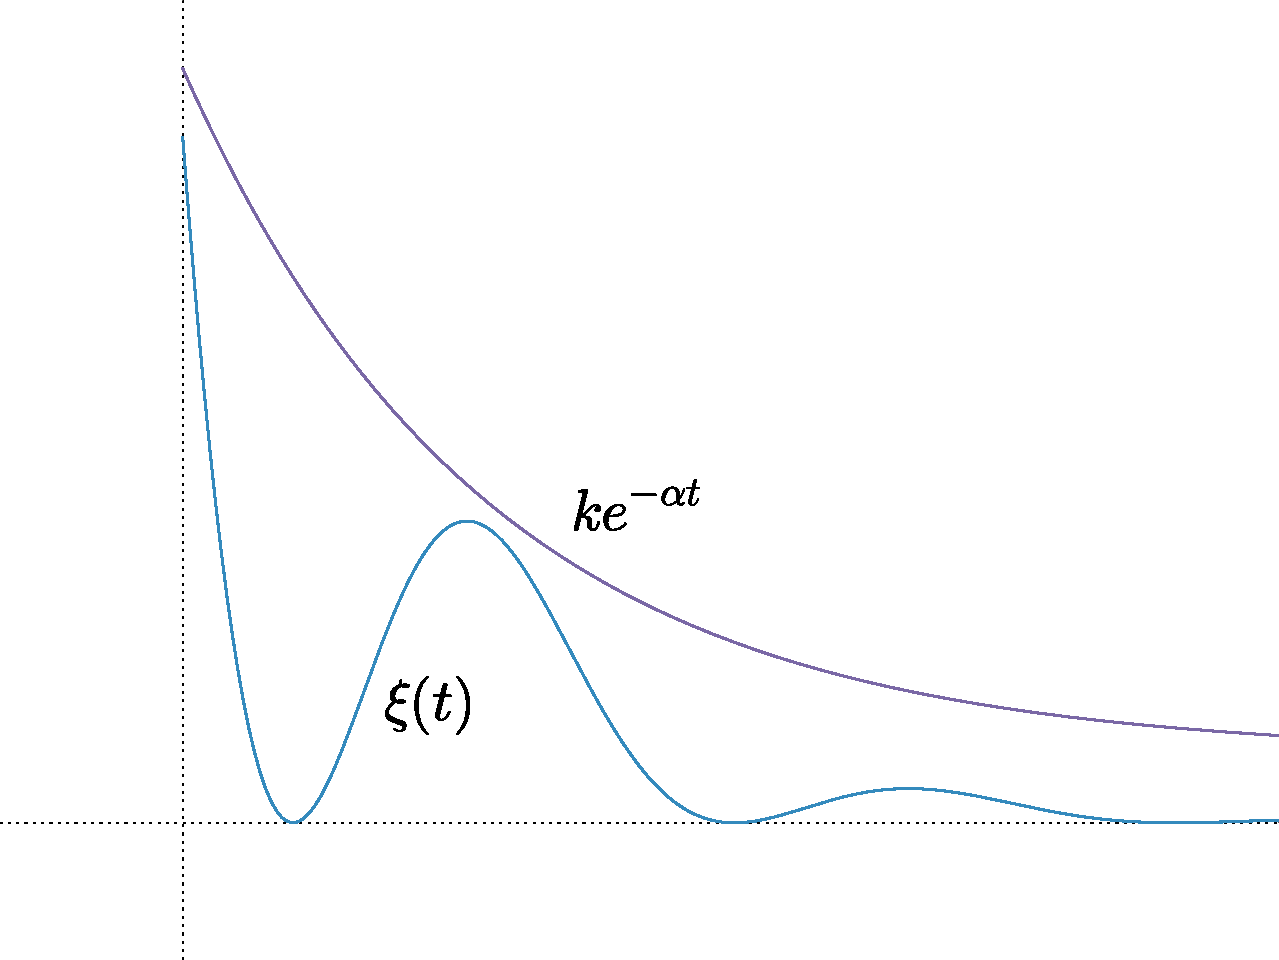
\includegraphics[width=\textwidth]{./imagenes/trayectoriafiltrada.pdf}
            \caption{\label{fig:trayectoriafiltrada}Comportamiento general de la señal filtrada acotado por exponencial.}
        \end{marginfigure}

        Puesto que $F(s)$ es un polinomio Hurwitz estable, entonces existe $k, \alpha \in \mathbbm{R}^+$, con $k > 0$ y $\alpha > 0$, tal que:

        \begin{equation*}
            |\xi(t)| \le k e^{- \alpha t} \quad \forall t \ge 0
        \end{equation*}

        por lo que para un $\alpha$ suficientemente grande, los comportamientos de las ecuaciones~\ref{eq:adap4} y~\ref{eq:adap1} será aproximadamente iguales.

        Desarrollando la ecuación~\ref{eq:adap4} se obtiene el siguiente regresor lineal:

        \begin{equation}
            y_f^{(n)}(t) = \theta^T \phi(t) + \xi(t)
        \end{equation}

        en donde:

        \begin{eqnarray} \label{eq:adap5}
            \theta^T & = & \begin{pmatrix} a_1 & \dots & a_n & b_0 & \dots & b_m \end{pmatrix} \in \mathbbm{R}^{n+m+1} \nonumber \\
            \phi^T & = & \begin{pmatrix} -y_f^{(n-1)} & \dots & -y_f & u_f^{(m)} & \dots & u_f \end{pmatrix} \in \mathbbm{R}^{n+m+1}
        \end{eqnarray}

        a los que llamamos vector de parametros y vector de mediciones.

        Note que las derivadas sucesivas de $y_f(t)$ y $u_f(t)$, se obtienen directamente de los filtros de las ecuaciones~\ref{eq:adap3}.

        \begin{figure}
            \centering
            \resizebox{\textwidth}{!}{
            \tikzstyle{block} = [draw, rectangle, minimum height=2.25em, minimum width=2.25em]

            \begin{tikzpicture}[auto, node distance=1.1cm, >=latex']
                \node [input, name=entrada] {};
                \node [block, right of=entrada] (uno) {$1$};
                \node [sum, right of=uno] (s1) {$+$};
                \node [block, right of=s1] (int1) {$\int$};
                \node [inner sep=0,minimum size=0,right of=int1] (xn) {};
                \node [block, right of=xn] (int2) {$\int$};
                \node [inner sep=0,minimum size=0,right of=int2] (xn1) {};
                \node [block, draw=none, right of=xn1] (vacio) {$\dots$};
                \node [inner sep=0,minimum size=0,right of=vacio] (x3) {};
                \node [block, right of=x3] (int3) {$\int$};
                \node [inner sep=0,minimum size=0,right of=int3] (x2) {};
                \node [block, right of=x2] (int4) {$\int$};
                \node [inner sep=0,minimum size=0,right of=int4] (x1) {};
                \node [output, right of=x1] (salida) {};

                \node [block, below of=int1] (a1) {$-f_1$};
                \node [block, below of=a1] (a2) {$-f_2$};
                \node [block, draw=none, below of=a2] (avacio) {$\vdots$};
                \node [block, below of=avacio] (an1) {$-f_{n-1}$};
                \node [block, below of=an1] (an) {$-f_n$};

                \draw [->] (entrada) -- node[name=u] {$x$} (uno);
                \draw [->] (uno)     -- (s1);
                \draw [->] (s1)      -- (int1);
                \draw [->] (int1)    -- node[name=xn] {$x^{(n)}$} (int2);
                \draw [->] (int2)    -- node[name=xn1] {$x^{(n-1)}$} (vacio);
                \draw [->] (vacio)   -- node[name=x3] {$x^{(3)}$} (int3);
                \draw [->] (int3)    -- node[name=x2] {$x^{(2)}$} (int4);
                \draw [->] (int4)    -- node[name=x1] {$x'$} (salida);

                \draw [->] (xn)  |- (a1);
                \draw [->] (xn1) |- (a2);
                \draw [->] (x2)  |- (an1);
                \draw [->] (x1)  |- (an);

                \draw [->] (a1)  -| (s1.324);
                \draw [->] (a2)  -| (s1.288);
                \draw [->] (an1) -| (s1.252);
                \draw [->] (an)  -| (s1.216);
            \end{tikzpicture}}
            \caption{\label{dia:adap5}Diagrama de bloques de un filtro para el regresor lineal.}
        \end{figure}

%-------------------------------------------------------------------------------
%	EMPIEZA SECCION
%-------------------------------------------------------------------------------

    \newpage
    \section{Algoritmo de identificación en linea}

        Un algoritmo de identificación es un procedimiento para estimar el vector de parámetros $\theta$ mediante la minimización de un criterio predeterminado.

        Se consideran dos tipos de algoritmo de identificación a saber:

        \begin{enumerate}
            \item Algoritmo tipo gradiente
            \item Algoritmo de mínimos cuadrados
        \end{enumerate}

%-------------------------------------------------------------------------------

        \subsection{Algoritmo tipo gradiente}

            \begin{problema}
                Encontrar el vector de parametros estimados $\theta(t)$, que minimice al siguiente criterio:

                \begin{equation}
                    J \left( \theta(t) \right) = \frac{1}{2} e^2 \left( \theta(t) \right) \ge 0
                \end{equation}

                donde:

                \begin{eqnarray}
                    e \left( \theta(t) \right) & = & \theta^T(t) \phi(t) - y_f^{(n)}(t) \nonumber \\
                    & = & \tilde{\theta}^T(t) \phi(t) = \phi^T(t) \tilde{\theta}(t)
                \end{eqnarray}

                y $\tilde{\theta}$ la definimos como:

                \begin{equation}
                    \tilde{\theta}(t) = \theta(t) - \theta
                \end{equation}

                A $e \left( \theta(t) \right)$ se le conoce como error de estimación y a $\tilde{\theta}(t)$ se le conoce como error paramétrico.
            \end{problema}

            Para resolver este problema derivemos el criterio $J(t)$ con respecto al tiempo:

            \begin{equation} \label{eq:adap6}
                \frac{d J(t)}{dt} = \frac{\partial J(t)}{\partial \theta(t)} \frac{d \theta(t)}{dt} = e(t) \frac{\partial e(t)}{\partial \theta(t)}^T \frac{d \theta(t)}{dt}
            \end{equation}

            para que $J(t)$ decrezca, se propone:

            \begin{equation}\label{eq:adap7}
                \frac{d \theta(t)}{dt} = -k e(t) \frac{\partial e(\theta(t))}{\partial \theta(t)} \text{ con } k > 0
            \end{equation}

            en efecto, de las ecuaciones~\ref{eq:adap6} y~\ref{eq:adap7} se tiene que:

            \begin{equation*}
                \frac{d J(t)}{dt} = -k e^2(t) \frac{\partial e(\theta(t))}{\partial \theta(t)}^T \frac{\partial e(\theta(t))}{\partial \theta(t)} \le 0 \quad \forall t \ge 0
            \end{equation*}

            lo cual implica que

            \begin{equation}
                J(t + T) \le J(t) \quad \forall T > t \ge 0
            \end{equation}

            Este es un algoritmo de programación no lineal de paso descendente.
            De la ecuación~\ref{eq:adap5} y la ecuación~\ref{eq:adap7} se obtiene el algoritmo de identificación tipo gradiente:

            \begin{equation} \label{eq:adap7}
                \frac{d \theta(t)}{dt} = -k \phi(t)e(t)
            \end{equation}

            \missingfigure{Diagrama de bloques de un identificador de tipo gradiente}

            \begin{lema}
                El algoritmo tipo gradiente descrito en la ecuación~\ref{eq:adap5} y en la ecuación~\ref{eq:adap7} tiene las siguientes propiedades:

                \begin{enumerate}
                    \item $\tilde{\theta}^T(t + T) \tilde{\theta}(t + T) \le \tilde{\theta}^T(t) \tilde{\theta}(t)$ para todo $T > t \ge 0$
                    \item $\left| \tilde{\theta}^T(t) \tilde{\theta}(t) \right| < \infty$ para casi todo $t \ge 0$
                    \item $\int_0^{\infty} e^2(\tau) d\tau < \infty$ para todo $t > 0$
                \end{enumerate}

                A estas propiedades les llamamos error paramétrico no creciente, error paramétrico acotado, y energía de error de estimación acotada.
            \end{lema}

            \begin{proof}
                Sea la siguiente función de Lyapunov:

                \begin{equation*}
                    V(t) = \frac{1}{2} \tilde{\theta}^T(t) \tilde{\theta}(t) \ge 0 \quad \forall t \ge 0
                \end{equation*}

                Entonces, recordando las ecuaciones~\ref{eq:adap5} y~\ref{eq:adap7} tenemos que:

                \begin{eqnarray*}
                    \frac{d V(t)}{dt} & = & \tilde{\theta}^T(t) \frac{d \tilde{\theta}(t)}{dt} \\
                    & = & \tilde{\theta}^T(t) \frac{d \theta(t)}{dt} \\
                    & = & -k \tilde{\theta}^T(t) \phi(t) e(t) \\
                    & = & -k e^2(t) \quad \forall t \ge 0
                \end{eqnarray*}

                por lo que:

                \begin{equation*}
                    \frac{d V(t)}{dt} \le 0 \quad \forall t \ge 0
                \end{equation*}

                lo cual implica que:

                \begin{equation*}
                    V(t) = V(0) - k \int_0^t e^2(\tau) d\tau
                \end{equation*}

                y dado que $V(t) \ge 0$, se tiene que:

                \begin{equation*}
                    \int_0^t e^2(\tau) d\tau = \frac{1}{k} \left( V(0) - V(t) \right) \le \frac{1}{k} V(0)
                \end{equation*}

                es decir:

                \begin{equation*}
                    \int_0^t e^2(\tau) d\tau \le \infty
                \end{equation*}

                Puesto que $V(t) \ge 0$ y $\frac{dV}{dt} \le 0$ para todo $t \ge 0$, se tiene que:

                \begin{equation*}
                    V(t + T) \le V(t) \quad \forall T > t \ge 0
                \end{equation*}

                esto es:

                \begin{equation*}
                    \tilde{\theta}^T(t + T) \tilde{\theta}(t + T) \le \tilde{\theta}^T(t) \tilde{\theta}(t) \quad \forall T > t \ge 0
                \end{equation*}

                Finalmente, haciendo la siguiente asignación:

                \begin{equation*}
                    (t, T) \mapsto (0, t)
                \end{equation*}

                se obtiene que:

                \begin{equation*}
                    \tilde{\theta}^T(t) \tilde{\theta}(t) \le \tilde{\theta}^T(0) \tilde{\theta}(0) \text{ para casi todo } t \ge 0
                \end{equation*}
            \end{proof}

%-------------------------------------------------------------------------------

        \subsection{Algoritmo de mínimos cuadrados}

            \begin{problema}
                Se quiere encontrar el vector de parametros que minimice el criterio de la ecuación~\ref{eq:adap8}:

                \begin{equation} \label{eq:adap8}
                    J \left( \theta(t) \right) = \int_0^t \lambda(\tau) e^2 (t, \tau) d\tau
                \end{equation}

                en donde:

                \begin{eqnarray}
                    & 0 < \lambda(\tau) \le 1 & \nonumber \\
                    & e(t, \tau) = \theta^T(t) \phi(\tau) - y_f^{(n)}(\tau) & \tau \in [0, t]
                \end{eqnarray}
            \end{problema}

            De nuevo comenzamos derivando el criterio a minimizar $J \left( \theta(t) \right)$ con respecto a $\theta(t)$ e igualamos a $0$ para obtener:

            \begin{eqnarray*}
                \frac{\partial J \left( \theta(t) \right)}{\partial \theta(t)} & = & \int_0^t \lambda(\tau) 2 e(t, \tau)\frac{\partial e(t, \tau)}{\partial \theta(t)} d\tau \\
                & = & 2 \int_0^t \lambda(\tau) \left( \theta^T(t) \phi(\tau) - y_f^{(n)}(\tau) \right) \phi(\tau) d\tau = 0
            \end{eqnarray*}

            es decir:

            \begin{equation} \label{eq:adap9}
                \theta(t) = \left( \int_0^t \lambda(\tau) \phi(\tau) \phi^T(\tau) d\tau \right)^{-1} \int_0^t \lambda(\tau) \phi(\tau) y_f^{(n)}(\tau) d\tau
            \end{equation}

            por lo que primero notamos que la inversa de la matriz $\int_0^t \lambda(\tau) \phi(\tau) \phi^T(\tau) d\tau$ existe bajo la condición de excitación persistente:

            \begin{equation}
                \int_0^t \lambda(\tau) \phi(\tau) \phi^T(\tau) d\tau \ge \delta I > 0 \quad \delta > 0
            \end{equation}

            es decir, para una $\delta I$ definida positivamente, tenemos que $\int_0^t \lambda(\tau) \phi(\tau) \phi^T(\tau) d\tau - \delta I$ tiene que ser semidefinida positivamente para que la matriz tenga una inversa.

            Por otro lado, podemos ver que el Hessiano del criterio de minimización $J \left( \theta(t) \right)$ es:

            \begin{equation}
                \frac{\partial^2 J \left( \theta(t) \right)}{\partial \theta(t) \partial \theta^T(t)} = 2 \int_0^t \lambda(\tau) \phi(\tau) \phi^T(\tau) d\tau > 0
            \end{equation}

            Si ahora definimos las matriz $P(t)$:

            \begin{equation}
                P(t) = \left( \int_0^t \lambda(\tau) \phi(\tau) \phi^T(\tau) d\tau \right) ^{-1}
            \end{equation}

            se tiene que su derivada con respecto al tiempo de su inversa es:

            \begin{equation} \label{eq:adap10}
                \frac{d P^{-1}(t)}{dt} = \lambda(t) \phi(t) \phi^T(t)
            \end{equation}

            entonces la ecuación~\ref{eq:adap9} tiene la siguiente forma:

            \begin{equation} \label{eq:adap11}
                \theta(t) = P(t) \int_0^t \lambda(\tau) \phi(\tau) y_f^{(n)}(\tau) d\tau
            \end{equation}

            lo cual implica que su derivada será:

            \begin{equation} \label{eq:adap12}
                \frac{d \theta(t)}{dt} = \frac{d P(t)}{dt} \int_0^t \lambda(\tau) \phi(\tau) y_f^{(n)}(\tau) d\tau + \lambda(t) P(t) \phi(t) y_f^{(n)}(t)
            \end{equation}

            Si notamos que

            \begin{equation*}
                0 = \frac{dI}{dt} = \frac{dP(t) P^{-1}(t)}{dt} = \frac{dP(t)}{dt} P^{-1}(t) + P(t) \frac{dP^{-1}(t)}{dt}
            \end{equation*}

            podemos obtener de la ecuación~\ref{eq:adap10}:

            \begin{equation} \label{eq:adap13}
                \frac{d P(t)}{dt} = - \lambda(t) P(t) \phi(t) \phi^T(t) P(t)
            \end{equation}

            por lo que de las ecuaciones~\ref{eq:adap11},~\ref{eq:adap12} y~\ref{eq:adap13} tenemos:

            \begin{eqnarray*}
                \frac{d \theta(t)}{dt} & = & - \lambda(t) P(t) \phi(t) \phi^T(t) P(t) \int_0^t \lambda(\tau) \phi(\tau) y_f^{(n)}(\tau) d\tau + \lambda(t) P(t) \phi(t) y_f^{(n)}(t) \\
                & = & - \lambda(t) P(t) \phi(t) \phi^T(t) \theta(t) + \lambda(t) P(t) \phi(t) y_f^{(n)}(t) \\
                & = & - \lambda(t) P(t) \phi(t) \left( \phi^T(t) \theta(t) - y_f^{(n)}(t) \right)
            \end{eqnarray*}

            es decir:

            \begin{eqnarray}
                \frac{d \theta(t)}{dt} & = & - \lambda(t) P(t) \phi(t) e(t) \nonumber \\
                e(t) & = & \theta^T(t) \phi(t) - y_f^{(n)}(t) \nonumber \\
                \frac{d P(t)}{dt} & = & - \lambda(t) P(t) \phi(t) \phi^T(t) P(t)
            \end{eqnarray}

            Dado este algoritmo de identificación tipo gradiente se sabe que tendrá las siguientes propiedades:

            \begin{enumerate}
                \item
                    \begin{eqnarray*}
                        0 < & P(t) & \le P(0) \\
                        0 < & P^{-1}(0) & \le P(t) \quad \forall t \ge 0
                    \end{eqnarray*}

                \item
                    \begin{equation*}
                        \int_0^t || P(\tau) \phi(\tau) || d\tau \le \traza{P(0)}
                    \end{equation*}

                \item
                    \begin{equation*}
                        \lim_{t \to \infty} P(t) = P_{\infty}
                    \end{equation*}

                \item
                    \begin{equation*}
                        P^{-1}(t)\tilde{\theta}(t) = P^{-1}(0) \tilde{\theta}(0)
                    \end{equation*}

                \item
                    \begin{eqnarray*}
                        \int_0^tP^2(\tau) d\tau & \le & \tilde{\theta}^T(0)P^{-1}(0)\tilde{\theta}(0) \\
                        \lambda_{min} \left\{ P^{-1}(0) \right\} || \hat{\theta}(t) ||_2^2 & \le & \tilde{\theta}^T(0)P^{-1}(0) \tilde{\theta}(0) \\
                        \lim_{t \to \infty} \tilde{\theta}(t) & = & P_{\infty}P^{-1}(0)\tilde{\theta}(0)
                    \end{eqnarray*}

                \item
                    \begin{equation*}
                        \int_{nT}^{(n-1)T} \phi(\tau) \phi^T(\tau) d\tau \ge \delta I > 0 \implies \lim_{t \to \infty} \theta(t) = \theta
                    \end{equation*}
            \end{enumerate}

    \newpage
    \section{Ejemplo}

        Sea el sistema representado por la ecuación diferencial ordinaria:

        \begin{equation}
            M \left( \frac{d}{dt} \right) y(t) = N \left( \frac{d}{dt} \right) u(t)
        \end{equation}

        donde $M(s) = s + a_1$ y $N(s) = b_0 s + b_1$.
        Se desea realizar un control adaptable tal que se asigne al polo en lazo cerrado en $s = -1$, sin modificar al cero\footnote{Al eliminar al cero del sistema corremos el riesgo de que el algoritmo de identificación tienda a hacer $0$ nuestra entrada al sistema, por lo que como regla general no se modifican los ceros.}, esto es, se desea la función de transferencia:

        \begin{equation}
            \frac{y(s)}{r(s)} = \frac{b_0 s + b_1}{s + 1}
        \end{equation}

        \subsection{Control lineal}

            Resolvamos primero la ecuación Diofantina:

            \begin{equation*}
                \mathcal{S}(s) M(s) + \mathcal{R}(s) N(s) = Q_D(s)
            \end{equation*}

            en donde:

            \begin{eqnarray}
                M(s) & = & s + a_1 \quad \grado{M(s)} = n = 1 \\
                N(s) & = & b_0 s + b_1 \quad \grado{N(s)} = m = 1 \le n = 1 \\
                Q_D(s) & = & q_0 s + q_1 \quad \grado{Q_D(d)} = 1 \le 2n - 1 = 1 \\
                \mathcal{R}(s) & = & r_0 \quad \grado{\mathcal{R}(s)} = 0 \le n - 1 = 0 \\
                \mathcal{S}(s) & = & s_0 \quad \grado{\mathcal{S}(s)} = 0 \le n - 1 = 0
            \end{eqnarray}

            Note que en este caso no es necesario la observación de estado implicita, ya que solo se tiene un estado del sistema, la salida.
            Así pues, la ecuación Diofantina queda:

            \begin{equation*}
                s_0 (s + a_1) + r_0 (b_0 s + b_1) = (s + 1)
            \end{equation*}

            lo cual implica:

            \begin{eqnarray*}
                s_0 + r_0 b_0 & = & 1 \\
                s_0 a_1 + r_0 b_1 & = & 1
            \end{eqnarray*}

            es decir:

            \begin{equation*}
                \begin{pmatrix}
                    1 & b_0 \\
                    a_1 & b_1
                \end{pmatrix}
                \begin{pmatrix}
                    s_0 \\
                    r_0
                \end{pmatrix} =
                \begin{pmatrix}
                    1 \\
                    1
                \end{pmatrix}
            \end{equation*}

            y como los polinomios son primos relativos, esta matriz $S(M, N)$ tiene inversa, es decir:

            \begin{equation*}
                \det{S(M, N)} = b_1 - a_1 b_0 = b_0 \left( \frac{b_1}{b_0} - a_1 \right)
            \end{equation*}

            por lo que procedemos a sacar la inversa:

            \begin{equation*}
                S^{-1}(M, N) = \frac{1}{b_1 - a_1 b_0}
                \begin{pmatrix}
                    b_1 & -b_0 \\
                    -a_1 & 1
                \end{pmatrix}
            \end{equation*}

            y por lo tanto:

            \begin{equation*}
                \begin{pmatrix}
                    s_0 \\
                    r_0
                \end{pmatrix} = \frac{1}{b_1 - a_1 b_0}
                \begin{pmatrix}
                    b_1 & -b_0 \\
                    -a_1 & 1
                \end{pmatrix}
                \begin{pmatrix}
                    1 \\
                    1
                \end{pmatrix} = \frac{1}{b_1 - a_1 b_0}
                \begin{pmatrix}
                    b_1 - b_0 \\
                    1 - a_1
                \end{pmatrix}
            \end{equation*}

            por lo que la ley de control lineal es:

            \begin{equation*}
                u(s) = - \frac{\mathcal{R}(s)}{\mathcal{S}(s)} y(s) + \frac{1}{\mathcal{S}(s)} r(s)
            \end{equation*}

            es decir:

            \begin{equation}
                u(s) = - \frac{1 - a_1}{b_1 - b_0} y(s) + \frac{b_1 - a_1 b_0}{b_1 - b_0} r(s)
            \end{equation}

            \missingfigure{Diagrama de bloques de controlador lineal basado en la resolución de la ecuación Diofantina por medio de la matriz de Sylvester.}

        \subsection{Regresor lineal}

            Si escribimos la ecuación diferencial ordinaria con los polinomios $M \left( \frac{d}{dt} \right)$ y $N \left( \frac{d}{dt} \right)$, tendremos:

            \begin{equation*}
                \left( \frac{d}{dt} + a_1 \right) y(t) = \left( b_0 \frac{d}{dt} + b_1 \right) u(t)
            \end{equation*}

            Asi pues, sean las señales filtradas:

            \begin{eqnarray*}
                F \left( \frac{d}{dt} \right) u_f & = & u \\
                F \left( \frac{d}{dt} \right) y_f & = & y
            \end{eqnarray*}

            en donde $F(s) = s + \frac{1}{\epsilon}$ con $\epsilon > 0$.
            Entonces tenemos:

            \begin{equation*}
                y_f' = \theta^T \phi(t) + \xi(t)
            \end{equation*}

            en donde $\theta = \begin{pmatrix} a_1 \\ b_0 \\ b_1 \end{pmatrix}$ y $\phi = \begin{pmatrix} -y_f \\ u_f' \\ u_f \end{pmatrix}$ y las derivadas de las señales las podemos obtener de los filtros.

            \begin{marginfigure}
                \centering
                \resizebox{\textwidth}{!}{
                \tikzstyle{block} = [draw, rectangle, minimum height=3em, minimum width=3em]

                \begin{tikzpicture}[auto, node distance=2cm, >=latex']
                    \node [input, name=entrada] {};
                    \node [sum, right of=entrada] (suma) {$+$};
                    \node [block, right of=suma] (integral) {$\int$};
                    \node [output, right of=integral] (salida1) {};
                    \node [output, above of=salida1] (salida2) {};
                    \node [block, below of=integral] (retro) {$-\frac{1}{\epsilon}$};

                    \draw [->] (entrada) -- node[name=u] {$u(s)$} (suma);
                    \draw [->] (suma) -- node[name=e]{} (integral);
                    \draw [->] (integral) -- node[name=y] {$u_f(s)$} (salida1);
                    \draw [->] (y) |- (retro);
                    \draw [->] (e) |- node[name=ufp, pos=0.9] {$u_f'(s)$} (salida2);
                    \draw [->] (retro) -| (suma);
                \end{tikzpicture}}
                \caption{\label{dia:adap6}Diagrama de bloques de filtro de señal de entrada.}
            \end{marginfigure}

            \begin{marginfigure}
                \centering
                \resizebox{\textwidth}{!}{
                \tikzstyle{block} = [draw, rectangle, minimum height=3em, minimum width=3em]

                \begin{tikzpicture}[auto, node distance=2cm, >=latex']
                    \node [input, name=entrada] {};
                    \node [sum, right of=entrada] (suma) {$+$};
                    \node [block, right of=suma] (integral) {$\int$};
                    \node [output, right of=integral] (salida1) {};
                    \node [output, above of=salida1] (salida2) {};
                    \node [block, below of=integral] (retro) {$-\frac{1}{\epsilon}$};

                    \draw [->] (entrada) -- node[name=u] {$y(s)$} (suma);
                    \draw [->] (suma) -- node[name=e]{} (integral);
                    \draw [->] (integral) -- node[name=y] {$y_f(s)$} (salida1);
                    \draw [->] (y) |- (retro);
                    \draw [->] (e) |- node[name=ufp, pos=0.9] {$y_f'(s)$} (salida2);
                    \draw [->] (retro) -| (suma);
                \end{tikzpicture}}
                \caption{\label{dia:adap7}Diagrama de bloques de filtro de señal de salida.}
            \end{marginfigure}

        \subsection{Algoritmo de identificación}

            \paragraph{Algoritmo tipo gradiente}\mbox{}\\

                Para implementar el algoritmo de identificación de tipo gradiente tenemos que usar las ecuaciones encontradas:

                \begin{eqnarray*}
                    \hat{\theta}'(t) & = & -k \phi(t) e(t) \\
                    \begin{pmatrix}
                        \hat{a}_1(t) \\
                        \hat{b}_0(t) \\
                        \hat{b}_1(t)
                    \end{pmatrix}' & = & -k
                    \begin{pmatrix}
                        -y_f(t) \\
                        u_f'(t) \\
                        u_f(t)
                    \end{pmatrix} e(t)
                \end{eqnarray*}

                en donde:

                \begin{eqnarray}
                    e(t) & = & \hat{\theta}^T(t) \phi(t) - y_f'(t) \\
                    & = & \left( -\hat{a}_1(t) y_f(t) + \hat{b}_0 u_f'(t) + \hat{b}_1(t) u_f(t) \right)
                \end{eqnarray}

                asi pues, el diagrama de bloques de este algoritmo de identificación queda:

                \missingfigure{Diagrama de bloques de alogritmo de identificacion de tipo gradiente}

            \paragraph{Algoritmo de mínimos cuadrados}\mbox{}\\

                Para el algoritmo de mínimos cuadrados tenemos las siguientes ecuaciones:

                \begin{eqnarray}
                    \hat{\theta}'(t) & = & - P(t) \phi(t) e(t) \\
                    e(t) & = & \hat{\theta}^T(t) \phi(t) - y_f'(t) \\
                    P'(t) & = & - P(t) \phi(t) \phi^T(t) P(t)
                \end{eqnarray}

                por lo que para empezar, tenemos que encontrar el valor de $P(t)$ de la siguiente ecuación:

                \begin{equation*}
                    \frac{d}{dt}
                    \begin{pmatrix}
                        p_1 & p_2 & p_3 \\
                        p_2 & p_4 & p_5 \\
                        p_3 & p_5 & p_6
                    \end{pmatrix} = -
                    \begin{pmatrix}
                        p_1 & p_2 & p_3 \\
                        p_2 & p_4 & p_5 \\
                        p_3 & p_5 & p_6
                    \end{pmatrix} \phi(t) \phi^T(t)
                    \begin{pmatrix}
                        p_1 & p_2 & p_3 \\
                        p_2 & p_4 & p_5 \\
                        p_3 & p_5 & p_6
                    \end{pmatrix}
                \end{equation*}
